\chapter[Simulação TO-BE]{Simulação TO-BE}
\label{chap:simulacao}
	A simulação do processo TO-BE consiste em apresentar os dados para a modelagem do TO-BE na sua versão 5, que é a final, e a versão 1, que é a versão proposta inicialmente para o AS-IS.

	\section[Propriedades dos Cenários de Simulação]{Propriedades dos Cenários de Simulação}
	\label{sec:simulacao_cenario}
		\begin{itemize}
	\item{\textbf{Cenário 1}:
		\begin{itemize}
			\item{\textbf{Duração}: 30 Dias;}
			\item{\textbf{Unidade Básica de Medida}: Horas;}
			\item{\textbf{Instâncias Iniciadas}: 10.}
		\end{itemize}}
	\item{\textbf{Cenário 2}:
		\begin{itemize}
			\item{\textbf{Duração}: 30 Dias;}
			\item{\textbf{Unidade Básica de Medida}: Horas;}
			\item{\textbf{Instâncias Iniciadas}: 30.}
		\end{itemize}}
	\item{\textbf{Recursos Disponíveis}:
		\begin{itemize}
			\item{\textbf{Gerente}: 1;}
			\item{\textbf{Avaliador}: 5;}
			\item{\textbf{Empresa}: 10;}
		\end{itemize}}
\end{itemize}

	\section[Recuros e Tempo de Processamento do Cenário de Simulação]{Recuros e Tempo de Processamento do Cenário de Simulação}
	\label{sec:simulacao_tempo}
		\begin{table}[H]
	\centering
	\begin{tabular}{|p{5cm}|c|c|c|}
		\hline
		\textbf{Atividade} & \textbf{Recurso} & \textbf{Quantidade} & \textbf{Horas} \\ \hline
		Analisar viabilidade de participação & Analista & 1 & 4 \\ \hline
		Disponibilizar solicitação de participação no MOA & Gerente & 1 & 1 \\ \hline
		Enviar mensagem de erro de preenchimento à empresa & Analista & 1 & 0.16 \\ \hline
		Enviar resposta para empresa & Analista & 1 & 0.16 \\ \hline
		Preencher solicitação de participação no MOA & Empresa & 1 & 1 \\ \hline
		Receber mensagem de erro de preenchimento & Empresa & 1 & 0.16 \\ \hline
		Receber resposta sobre a viabilidade & Empresa & 1 & 0.16 \\ \hline
	\end{tabular}
	\caption[Recursos e Tempo de Processamento do Cenário do TO-BE Versão 01]{Recursos e Tempo de Processamento do Cenário do TO-BE Versão 01}
\end{table}

\begin{table}[H]
	\centering
	\begin{tabular}{|p{5cm}|c|c|c|}
		\hline
		\textbf{Atividade} & \textbf{Recurso} & \textbf{Quantidade} & \textbf{Horas} \\ \hline
		Analisar viabilidade de participação & Analista & 1 & 4 \\ \hline
		Atribuir solicitação para avaliação & Gerente & 1 & 1 \\ \hline
		Avaliar se é desejável corrigir & Empresa & 1 & 0.5 \\ \hline
		Consultar status da empresa & Empresa & 1 & 0.16 \\ \hline
		Disponibilizar solicitação de participação no MOA & Gerente & 1 & 2 \\ \hline
		Preencher solicitação de participação no MOA & Empresa & 1 & 2 \\ \hline
	\end{tabular}
	\caption[Recursos e Tempo de Processamento do Cenário do TO-BE Versão 05]{Recursos e Tempo de Processamento do Cenário do TO-BE Versão 05}
\end{table}

	\section[Resultado da Simulação]{Resultado da Simulação}
	\label{sec:simulacao_resultado}
		O tempo total médio do processo TO-BE v1 foi de 12,32 horas para o cenário 1 e 26,29 horas para o 2. A Figura \ref{fig:resultadostobevum} apresenta os resultados da simulação.
\begin{figure}[H]
	\centering
	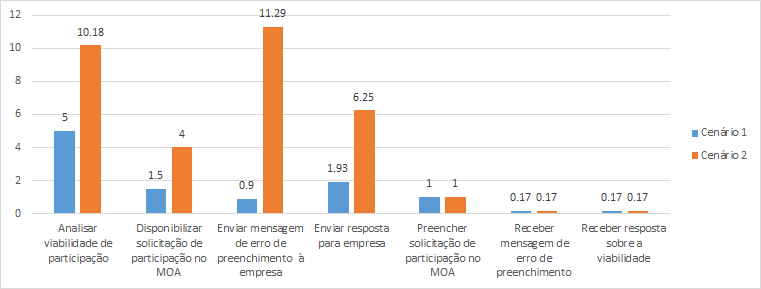
\includegraphics[scale=0.78]{resultado_tobe_v1_simulacao}
	\caption[Gráfico de Resultados da Simulação TO-BE Versão 01]{Gráfico de Resultados da Simulação TO-BE Versão 01.}
	\label{fig:resultadostobevum}
\end{figure}
O tempo total médio do processo TO-BE v5 foi de 15,48 horas para o cenário 1 e 36,37 horas para o 2. A Figura \ref{fig:resultadostobevcinco} apresenta os resultados da simulação.
\begin{figure}[H]
	\centering
	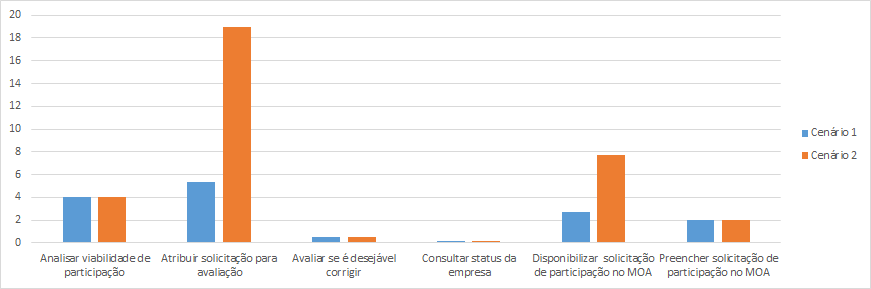
\includegraphics[scale=0.69]{resultado_tobe_v5_simulacao}
	\caption[Gráfico de Resultados da Simulação TO-BE Versão 05]{Gráfico de Resultados da Simulação TO-BE Versão 05.}
	\label{fig:resultadostobevcinco}
\end{figure}

	\section[Recursos]{Recursos}
	\label{sec:simulacao_recursos}
		\begin{figure}[H]
	\centering
	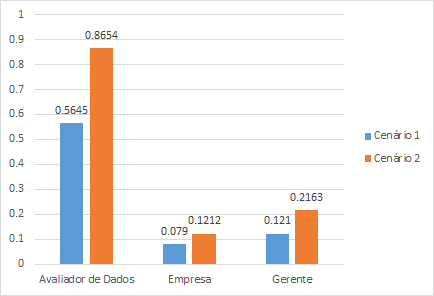
\includegraphics[scale=1]{recursos_tobe_v1_simulacao}
	\caption[Gráfico de Recursos da Simulação TO-BE Versão 01]{Gráfico de Recursos da Simulação TO-BE Versão 01.}
	\label{fig:recursostobevum}
\end{figure}

\begin{figure}[H]
	\centering
	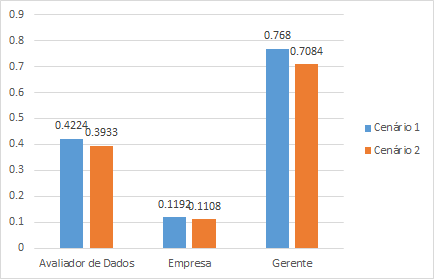
\includegraphics[scale=1]{recursos_tobe_v5_simulacao}
	\caption[Gráfico de Recursos da Simulação TO-BE Versão 05]{Gráfico de Recursos da Simulação TO-BE Versão 05.}
	\label{fig:recursostobevcinco}
\end{figure}

	\section[Análise do Resultado]{Análise do Resultado}
	\label{sec:simulacao_analise}
		A simulação para ambas as versões do TO-BE apresentaram valores consistentes para o tempo esperado para cada atividade no cenário 1. Para o cenário 2 os valores se apresentaram muito superiores para a versão 1, porém a versão 5 não se comportou da mesma maneira para suas atividade, evidenciando assim uma clara melhoria quanto à eficiência da modelagem proposta. 
\\ \indent Evidenciou-se um maior equilíbrio de utilização de recursos na versão 5 do que na 1 do TO-BE. Tal fato também se mostra verdadeiro quando equiparado à utilização de recursos do AS-IS. Em relação ao AS-IS, o avaliador teve um aumento médio de 584,84\%, a empresa teve um aumento de 53,19\%, e o gerente aumentou 114,71\% na média.
\\ \indent O processo TO-BE versão 5 apresentou uma média de horas de execução de 3,16 horas a mais para o cenário 1, e de 10,08 horas a mais para o 2. Este aumento se deu principalmente pela adicão tarefa do gerente “Atribuir solicitação para avaliação”. Devido a essa diferença de tempo não ser muito significativa e também o fato do processo ser executado com mais de 200 horas a menos do que o AS-IS, a versão 5 se mostrou a melhor para ser utilizada no processo de automação.